\documentclass[onecolumn,12pt]{IEEEtran}
\usepackage{amsmath, amssymb}
\usepackage{setspace}
\usepackage{graphicx}
\usepackage{geometry}
\usepackage{hyperref}
\usepackage{float}
\geometry{margin=1in}



\title{Warehouse Operations Simulation}
\author{Cameron LaVaughn}
\date{\today}

\begin{document}
\doublespacing
\maketitle

\section{Project Overview}

\subsection{Project Title}
Warehouse Operations and Logistics Simulation

\subsection{Domain}
Supply Chain and Logistics, with a focus on warehouse operations and automation.

\subsection{Problem Statement}
The Modern warehouses mostly rely on efficient order processing, inventory management, and automated material handling systems. This simulation will  aim to answer the following questions:
\begin{itemize}
    \item How do the different order arrival rates affect warehouse throughput?
    \item What are the impact of inventory placement strategies on order fulfillment time?
    \item How does robot routing efficiency influence overall warehouse performance?
\end{itemize}

\subsection{Scope}
This simulation will model internal warehouse operations within a single fulfillment center. It will include the storage zones, pick locations, autonomous mobile robots, and the order processing logic. The following elements are \textbf{out of scope}: supplier lead times, transportation between facilities, human labor variability, and equipment failures.

\section{System Description}

\subsection{System Components}
\begin{itemize}
    \item \textbf{Orders}: Arrival time, Number of Items, Priority
    \item \textbf{Inventory Items}: SKU, Quantity, Storage Location
    \item \textbf{Storage Locations}: Capacity and Occupancy
    \item \textbf{Robots}: position, Speed, Task Status
    \item \textbf{Warehouse Layout}: Graph of aisles and Nodes
\end{itemize}

\subsection{System Dynamics}
 The Orders will arrive stochastically and are queued for processing. Inventory is checked and the tasks are assigned to the robots. Robots will navigate through the warehouse using shortest-path routing to retrieve the items and they will deliver them to packing stations. System state evolves based on events such as order arrivals, robot movements, and order completion.

\subsection{Core Models and Algorithms}
\begin{enumerate}
    \item \textbf{Inventory Model}: A continuous-review $(Q, R)$ inventory policy where the replenishment occurs when stock falls below a reorder point.
    \item \textbf{Shortest Path Routing}: Robot navigation uses Dijkstra’s algorithm to minimize the travel distance.
    \item \textbf{Task Assignment}: Orders are assigned to the robots using a priority-based heuristic.
\end{enumerate}

\subsection{Assumptions}
\begin{itemize}
    \item Robots move at a constant speed with no collisions.
    \item Inventory data is accurate and real-time.
    \item Order arrivals follow a stationary stochastic process.
\end{itemize}

\section{Implementation Approach}

\subsection{Programming Language}
Python is used because of its strong support for simulation and optimization.

\subsection{Development Environment}
\begin{itemize}
    \item Python 3
    \item SimPy
    \item NetworkX
    \item NumPy, Pandas
    \item Matplotlib
\end{itemize}

\subsection{Simulation Type}
Discrete-event simulation.

\subsection{Data Collection Plan}
\begin{itemize}
    \item Order fulfillment time
    \item Warehouse throughput
    \item Storage efficiency
    \item Robot utilization
\end{itemize}

\section{Literature Review}

\subsection{Core Models and Algorithms}

This section will review the foundational models and algorithms used in warehouse operations and logistics simulations. At least five established sources inform the design of this project.

\subsubsection{Inventory Control Models -- $(Q, R)$ Policy}
\textbf{Source:} Silver, Pyke, and Peterson, \emph{Inventory Management and Production Planning and Scheduling}.

This work presents the continuous-review inventory models where a fixed quantity $Q$ is reordered once inventory drops below a reorder point $R$. These models balance holding costs and stockout risks.

\textbf{Application to Project:} The $(Q, R)$ model governs the SKU replenishment logic in the warehouse.

\textbf{Adaptation:} The lead times are assumed to be deterministic and replenishment occurs instantaneously to isolate internal warehouse behavior.

\subsubsection{Poisson Order Arrival Modeling}
\textbf{Source:} Gross and Harris, \emph{Fundamentals of Queueing Theory}.

Poisson processes are widely used to model random arrivals in service systems.

\textbf{Application to Project:} The customer orders arrive according to a Poisson process.

\textbf{Adaptation:} Arrival rates will remain constant per simulation run.

\subsubsection{Shortest Path Algorithms for Routing}
\textbf{Source:} Dijkstra, E. W. (1959). \emph{A Note on Two Problems in Connexion with Graphs}.

Dijkstra’s algorithm computes shortest paths in weighted graphs.

\textbf{Application to Project:} Warehouse aisles are modeled as a graph for robot navigation.

\textbf{Adaptation:} Edge weights represent distance only, ignoring congestion.

\subsubsection{Warehouse Order Picking Systems}
\textbf{Source:} de Koster, Le-Duc, and Roodbergen (2007). \emph{Design and Control of Warehouse Order Picking}.

This survey examines the strategy selection and layout design.

\textbf{Application to a project:} Influences task assignment and layout abstraction.

\textbf{Adaptation:} Human pickers are replaced by autonomous robots.

\subsubsection{Discrete-Event Simulation}
\textbf{Source:} Banks et al., \emph{Simulation of discrete}.

This textbook formalizes event-driven simulation techniques.

\textbf{Application to Project:} Defines the simulation architecture.

\textbf{Adaptation:} Events are limited to order arrivals, robot dispatch, retrieval, and completion.

\subsection{Related Work}

Existing warehouse simulations such as academic robotic fulfillment models and industry research platforms influenced this design. These systems commonly use the discrete-event frameworks, graph-based routing, and task queues. This project will adapt to these approaches into a simplified, educational simulation while preserving realistic system dynamics.

\section{UML Diagrams}

\subsection{Class Diagram}

This class diagram represents the primary simulation entities and their relationships:

\begin{figure}[h!]
    \centering
    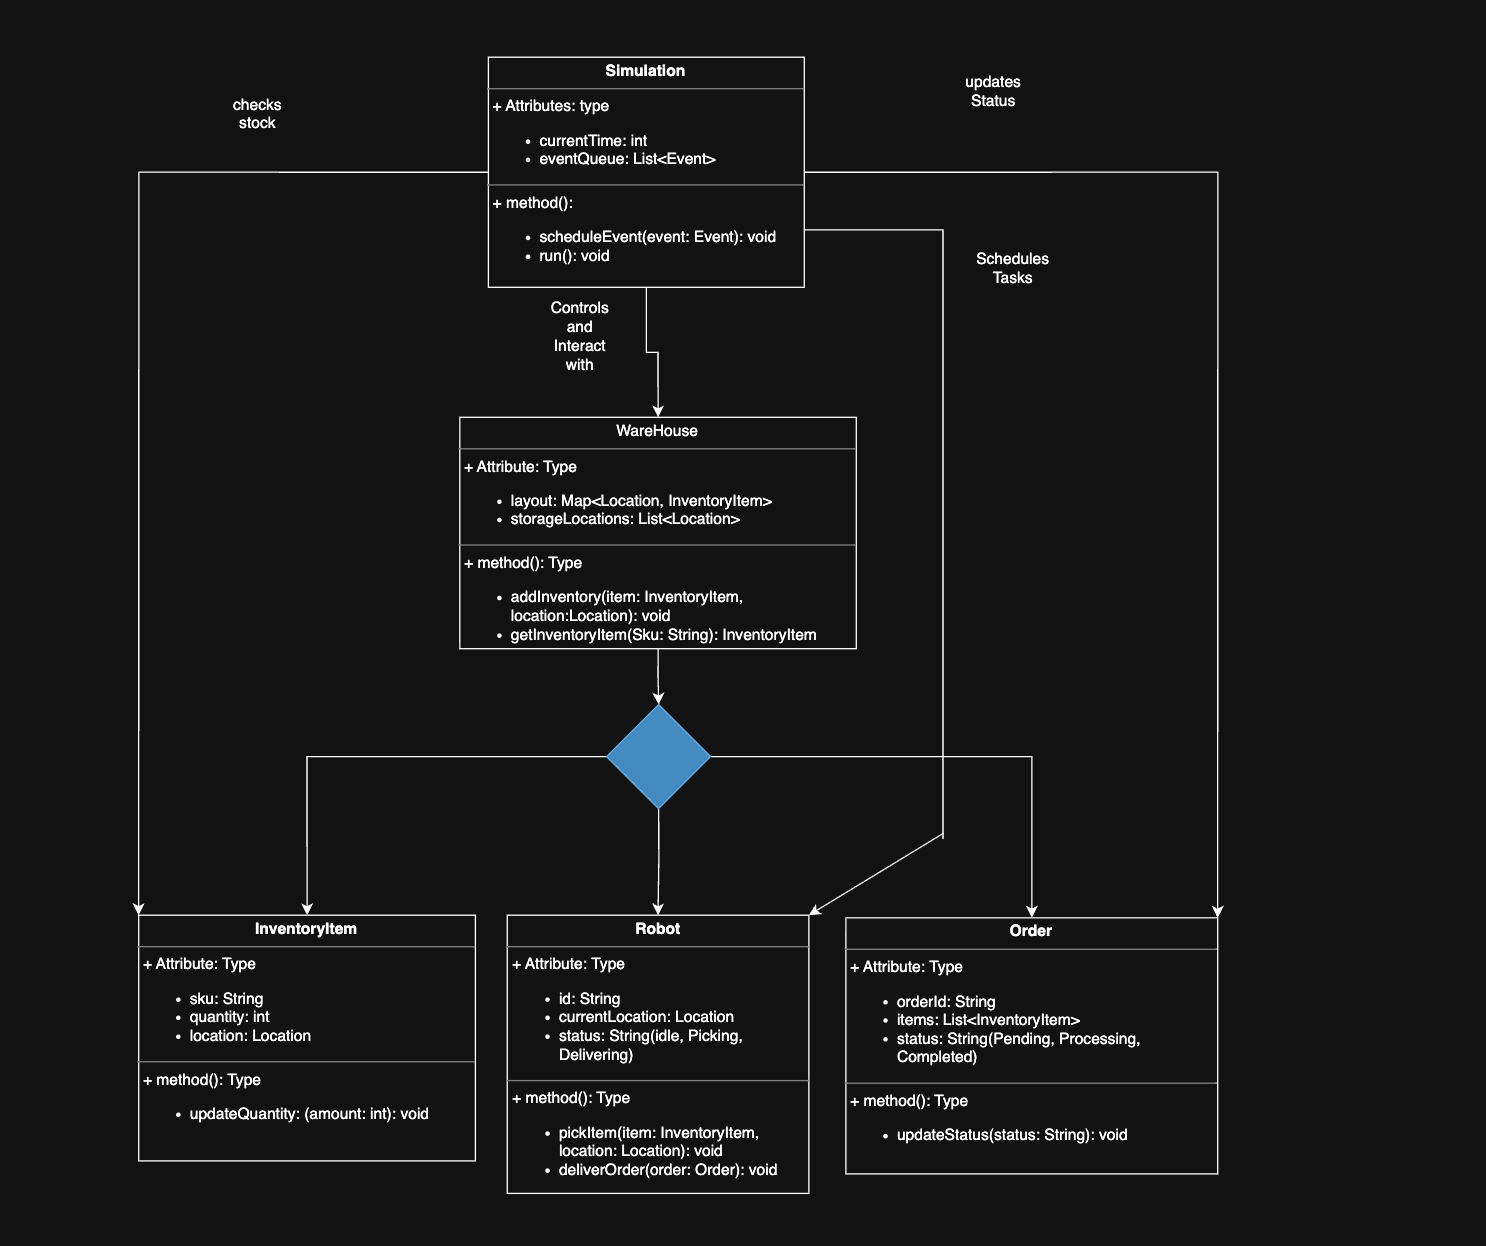
\includegraphics[width=0.8\textwidth]{images/Class Diagram.png}
    \caption{UML Class Diagram of the Warehouse Simulation.}
    \label{fig:class_diagram}
\end{figure}


\begin{itemize}
    \item \textbf{Simulation}: Controls event scheduling and the global time
    \item \textbf{Order}: Stores the order attributes and status
    \item \textbf{InventoryItem}: Tracks SKU quantities and their locations
    \item \textbf{Robot}: Executes picking and delivery tasks
    \item \textbf{Warehouse}: Maintains the layout and storage locations
\end{itemize}

The Warehouse class composes the Robots, InventoryItems, and Orders. The Simulation class arranges interactions among all the components.

\subsection{Sequence Diagram}
\begin{figure}[H]
    \centering
    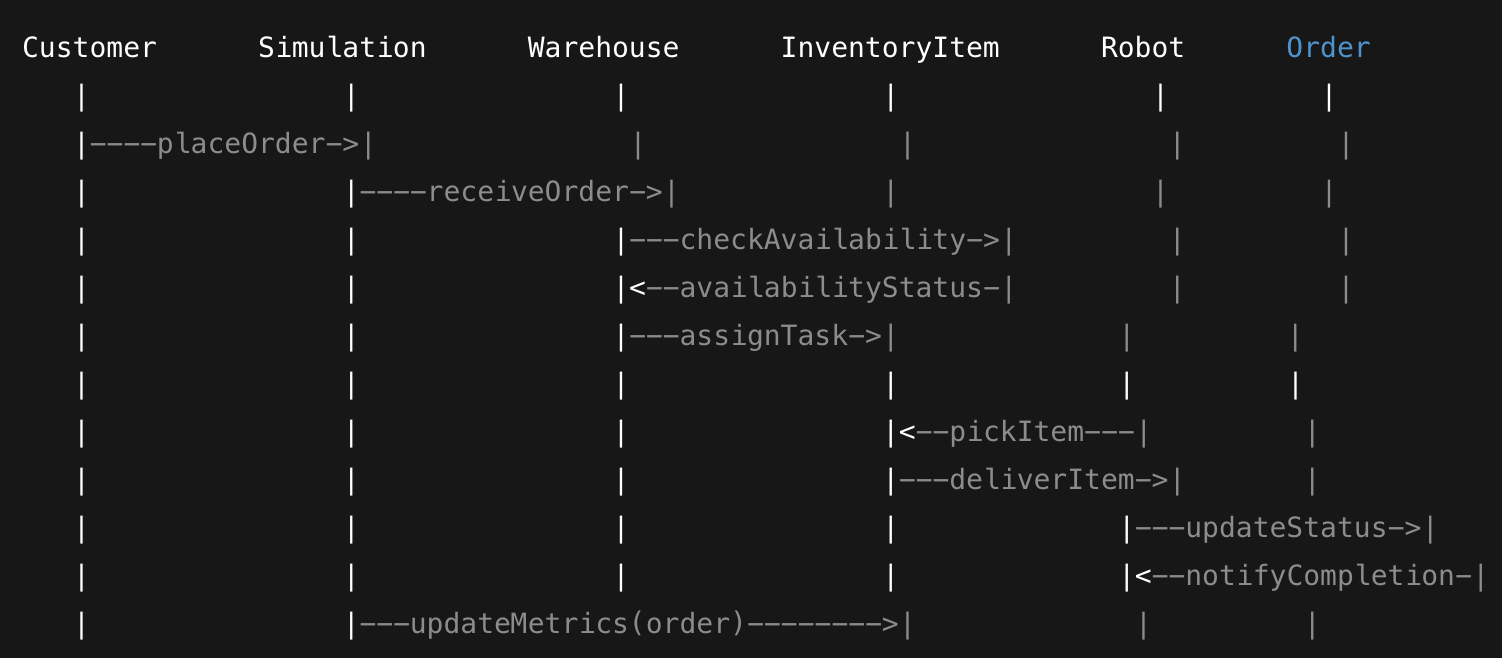
\includegraphics[width=0.8\textwidth]{images/Sequence Diagram.png }
    \caption{Sequence Diagram of the Warehouse Simulation.}
    \label{fig:sequence_diagram}
\end{figure}
This  sequence diagram is used to represent the discrete-event flow:


\begin{enumerate}
    \item Order arrives
    \item Inventory availability is checked
    \item Robot is assigned
    \item Robot computes shortest path
    \item Item is retrieved and delivered
    \item Order completion updates metrics
\end{enumerate}

This diagram reflects the event-driven nature of the simulation.


\section{References}

\begin{thebibliography}{99}

\bibitem{gu2007}
J. Gu, M. Goetschalckx, and L. F. McGinnis,
``Research on warehouse operation: A comprehensive review,''
\textit{European Journal of Operational Research},
vol. 177, no. 1, pp. 1--21, 2007.

\bibitem{dijkstra1959}
E. W. Dijkstra,
``A note on two problems in connexion with graphs,''
\textit{Numerische Mathematik},
vol. 1, no. 1, pp. 269--271, 1959.

\bibitem{silver2016}
E. A. Silver, D. F. Pyke, and R. Peterson,
\textit{Inventory Management and Production Planning and Scheduling},
3rd ed. Hoboken, NJ, USA: Wiley, 2016.

\bibitem{simpy}
T. Hoel and S. R. Schilling,
``SimPy: Simulation in Python,''
\textit{Journal of Open Source Software},
vol. 2, no. 16, pp. 1--3, 2017.

\bibitem{wurman2008}
P. R. Wurman, R. D’Andrea, and M. Mountz,
``Coordinating hundreds of cooperative, autonomous vehicles in warehouses,''
\textit{AI Magazine},
vol. 29, no. 1, pp. 9--20, 2008.

\end{thebibliography}

\end{document}
